\documentclass[11pt, a4paper, reqno]{scrartcl}

\usepackage[utf8]{inputenc}
\usepackage{a4wide}
\usepackage{libertine}
\usepackage{graphicx}
\usepackage{listings}
\usepackage{xcolor}
\usepackage{float}
\usepackage{amsmath}

% for latex output of pandas
\usepackage{booktabs}

\begin{document}
    \title{Exercise No. 1}
    \author{David Bubeck, Pascal Becht, Patrick Nisbl\`e}
    \maketitle
    
    \lstset{
        language=Python,
        backgroundcolor=\color{gray!10},
        numbers=left,
        captionpos=b,
        xleftmargin=\parindent,
        basicstyle=\footnotesize\sffamily,
        keywordstyle=\bfseries\color{green!40!black},
        commentstyle=\itshape\color{purple!40!black},
        identifierstyle=\color{blue!60!black},
        stringstyle=\color{orange}
    }

    \newpage
    \section*{2 - Numerical Integration}
    \subsection*{a)}
    
    \lstinputlisting[language=Python,
                     lastline=17, 
                     caption={
                        h
                     }]{01-2a.py}
    \begin{figure}[H]
        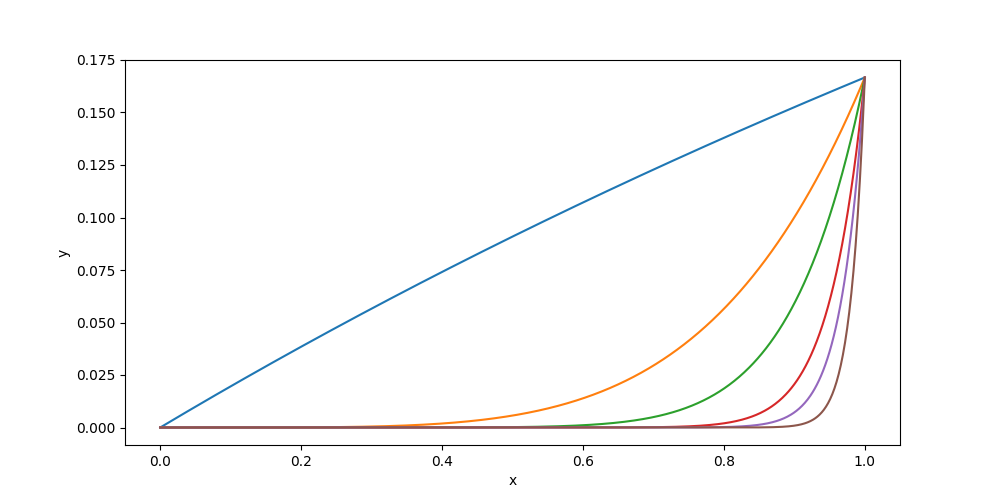
\includegraphics[width=.7\paperwidth]{01-2a}
        \caption{h}
    \end{figure}

    \newpage
    \subsection*{b)}
    
    \lstinputlisting[lastline=25]{01-2b.py}w2
    \begin{figure}[H]
        \centering
        \begin{tabular}{lrr}
\toprule
{} &     n &    $y_n(5.0)$ \\
\midrule
0  &   0.0 &  1.000000e+01 \\
1  &  10.0 & -4.990909e+01 \\
2  &  11.0 &  2.496288e+02 \\
3  &  12.0 & -1.248067e+03 \\
4  &  13.0 &  6.240407e+03 \\
5  &  14.0 & -3.120197e+04 \\
6  &  15.0 &  1.560099e+05 \\
7  &  16.0 & -7.800494e+05 \\
8  &  17.0 &  3.900247e+06 \\
9  &  18.0 & -1.950124e+07 \\
10 &  19.0 &  9.750618e+07 \\
11 &  20.0 & -4.875309e+08 \\
12 &  21.0 &  2.437654e+09 \\
13 &  22.0 & -1.218827e+10 \\
14 &  23.0 &  6.094136e+10 \\
15 &  24.0 & -3.047068e+11 \\
16 &  25.0 &  1.523534e+12 \\
17 &  26.0 & -7.617670e+12 \\
18 &  27.0 &  3.808835e+13 \\
19 &  28.0 & -1.904418e+14 \\
20 &  29.0 &  9.522088e+14 \\
21 &  30.0 & -4.761044e+15 \\
\bottomrule
\end{tabular}
    
    \end{figure}

    \newpage
    \subsection*{c)}
    
    
    
    
\end{document}